\section{PG Algebra}

\subsection{Abstract}

One of the difficulties in designing modern hardware systems is the
necessity to comprehend and to deal with a very large number of system
configurations, operational modes, and behavioural scenarios. It is
often infeasible to consider and specify each individual mode explicitly,
and one needs methodologies and tools to exploit similarities between
the individual modes and work with groups of modes rather than individual
ones. The modes and groups of modes have to be managed in a compositional
way: the specification of the system should be composed from specifications
of its blocks. This includes both structural and behavioural composition.
Furthermore, one should be able to transform and optimise the specifications
in a fully formal and natural way.

In this paper we propose a new formalism, called Parameterised Graphs.
It extends the existing Conditional Partial Order Graphs (CPOGs) formalism
in several ways. First, it deals with general graphs rather than just
partial orders. Moreover, it is fully compositional. To achieve this
we introduce an algebra of Parameterised Graphs by specifying the
equivalence relation by a set of axioms, which is proved to be sound,
minimal and complete. This allows one to manipulate the specifications
as algebraic expressions using the rules of this algebra. We demonstrate
the usefulness of the developed formalism on two case studies coming
from the area of microelectronics design.

\subsection{Introduction}

\thispagestyle{plain}While the complexity of modern hardware exponentially
increases due to Moore's law, the time-to-market is reducing. The
number of available transistors on chip exceeds the capabilities of
designers to meaningfully use them: this \emph{design productivity
gap} is a major challenge in the microelectronics industry~\cite{2009_design_itrs}.
One of the difficulties of the design is the necessity to comprehend
and to deal with a very large number of system configurations, operational
modes, and behavioural scenarios. The contemporary systems often have
abundant functionality and enjoy features like fault-tolerance, dynamic
reconfigurability, power management, all of which greatly increase
the number of possible modes of operation. Hence, it is often infeasible
to consider and specify each individual mode explicitly, and one needs
methodologies and tools to exploit similarities between the individual
modes and work with groups of modes rather than individual ones. The
modes and groups of modes have to be managed in a compositional way:
the specification of the system should be composed from specifications
of its blocks. This includes both structural and behavioural composition.
Furthermore, one should be able to transform and optimise the specifications
in a fully formal and natural way.

In this paper we continue the work started in~\cite{2010_mokhov_ieee},
where a formal model, called Conditional Partial Order Graphs (CPOGs),
was introduced. It allowed to represent individual system configurations
and operational modes as annotated graphs, and to overlay them exploiting
their similarities. However, the formalism lacked the compositionality
and the ability to compare and transform the specifications in a formal
way. In particular, CPOGs always represented the specification as
a `flat' structure (similar to the canonical form defined in Section~\ref{sec:Parametrised-Graphs}),
hence a hierarchical representation of a system as a composition of
its components was not possible. We extend this formalism in several
ways:
\begin{itemize}
\item We move from the graphs representing partial orders to general graphs.
Nevertheless, if partial orders are the most natural way to represent
a certain aspect of system, this still can be handled.
\item The new formalism is fully compositional.
\item We describe the equivalence relation between the specifications as
a set of axioms, obtaining an algebra. This set of axioms is proved
to be sound, minimal and complete.
\item The developed formalism allows to manipulate the specifications as
algebraic expressions using the rules of the algebra. In a sense this
can be viewed as adding a syntactic level to the semantic representation
of specifications, and is akin to the relationship between digital
circuits and Boolean algebra.
\end{itemize}
We demonstrate the usefulness of the developed formalism on two case
studies. The first one is concerned with development of a phase encoding
controller, which represents information by the order of arrival of
signals on $n$ wires. As there are $n!$ possible arrival orders,
there is a challenge to specify the set of corresponding behavioural
scenarios in a compact way. The proposed formalism not only allows
to solve this problem, but also does it in a compositional way, by
obtaining the final specification as a composition of fixed-size fragments
describing the behaviours of pairs of wires (the latter was impossible
with CPOGs).

\begin{figure*}
\begin{centering}
\hfill{}\subfloat[Graph $G_{1}$]{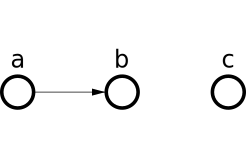
\includegraphics[scale=0.5]{fig/graph_3}

}\hfill{}\hfill{}\subfloat[Graph $G_{2}$]{
\includegraphics[scale=0.5]{fig/graph_4}

}\hfill{}\hfill{}\subfloat[Graph $G_{1}+G_{2}$]{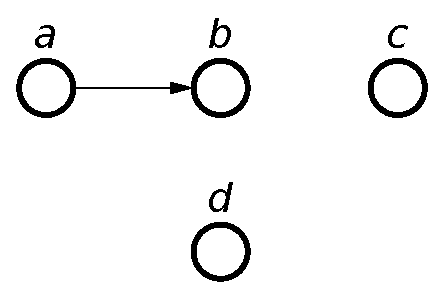
\includegraphics[scale=0.5]{fig/graph_overlay_3_4}

}\hfill{}\hfill{}\subfloat[Graph $G_{1}\rightarrow G_{2}$]{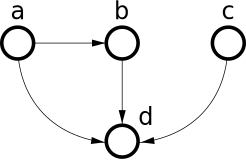
\includegraphics[scale=0.5]{fig/graph_sequence_3_4}

}\hfill{}
\par\end{centering}

\caption{Overlay and sequence example (no common vertices)\label{fig:Overlay-and-sequence-no-common}}
\end{figure*}


\begin{figure*}
\begin{centering}
\hfill{}\subfloat[Graph $G_{1}$]{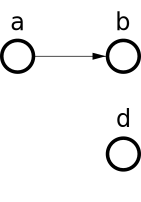
\includegraphics[scale=0.5]{fig/graph_1}

}\hfill{}\hfill{}\subfloat[Graph $G_{2}$]{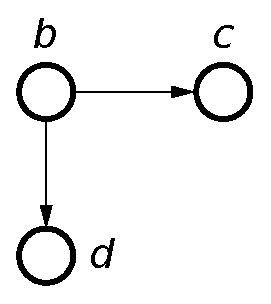
\includegraphics[scale=0.5]{fig/graph_2}

}\hfill{}\hfill{}\subfloat[Graph $G_{1}+G_{2}$]{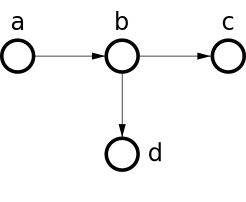
\includegraphics[scale=0.5]{fig/graph_overlay_1_2}

}\hfill{}\hfill{}\subfloat[Graph $G_{1}\rightarrow G_{2}$]{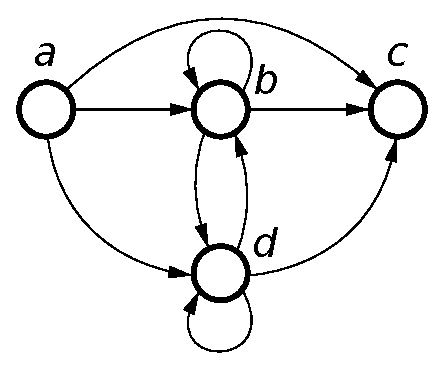
\includegraphics[scale=0.5]{fig/graph_sequence_1_2}

}\hfill{}
\par\end{centering}

\caption{Overlay and sequence example (common vertices)\label{fig:Overlay-and-sequence}}
\end{figure*}


The second case study is concerned with designing a microcontroller
for a simple processor. The processor can execute several classes
of instructions, and each class is characterised by a specific execution
scenario of the operational units of the processor. In turn, the scenarios
of conditional instructions have to be composed of sub-scenarios corresponding
to the current value of the appropriate ALU flag. The overall specification
of the microcontroller is then obtained algebraically, by composing
scenarios of each class of instructions.

The full version of this paper can be found in the technical report~\cite{2011_mokhov_pg}
(available on-line), where also the missing proofs can be found.

